\section{Background}
% \label{Motivation}
% \label{subsec:motivation-objective}
% 
\begin{figure}[H]
    \centering
  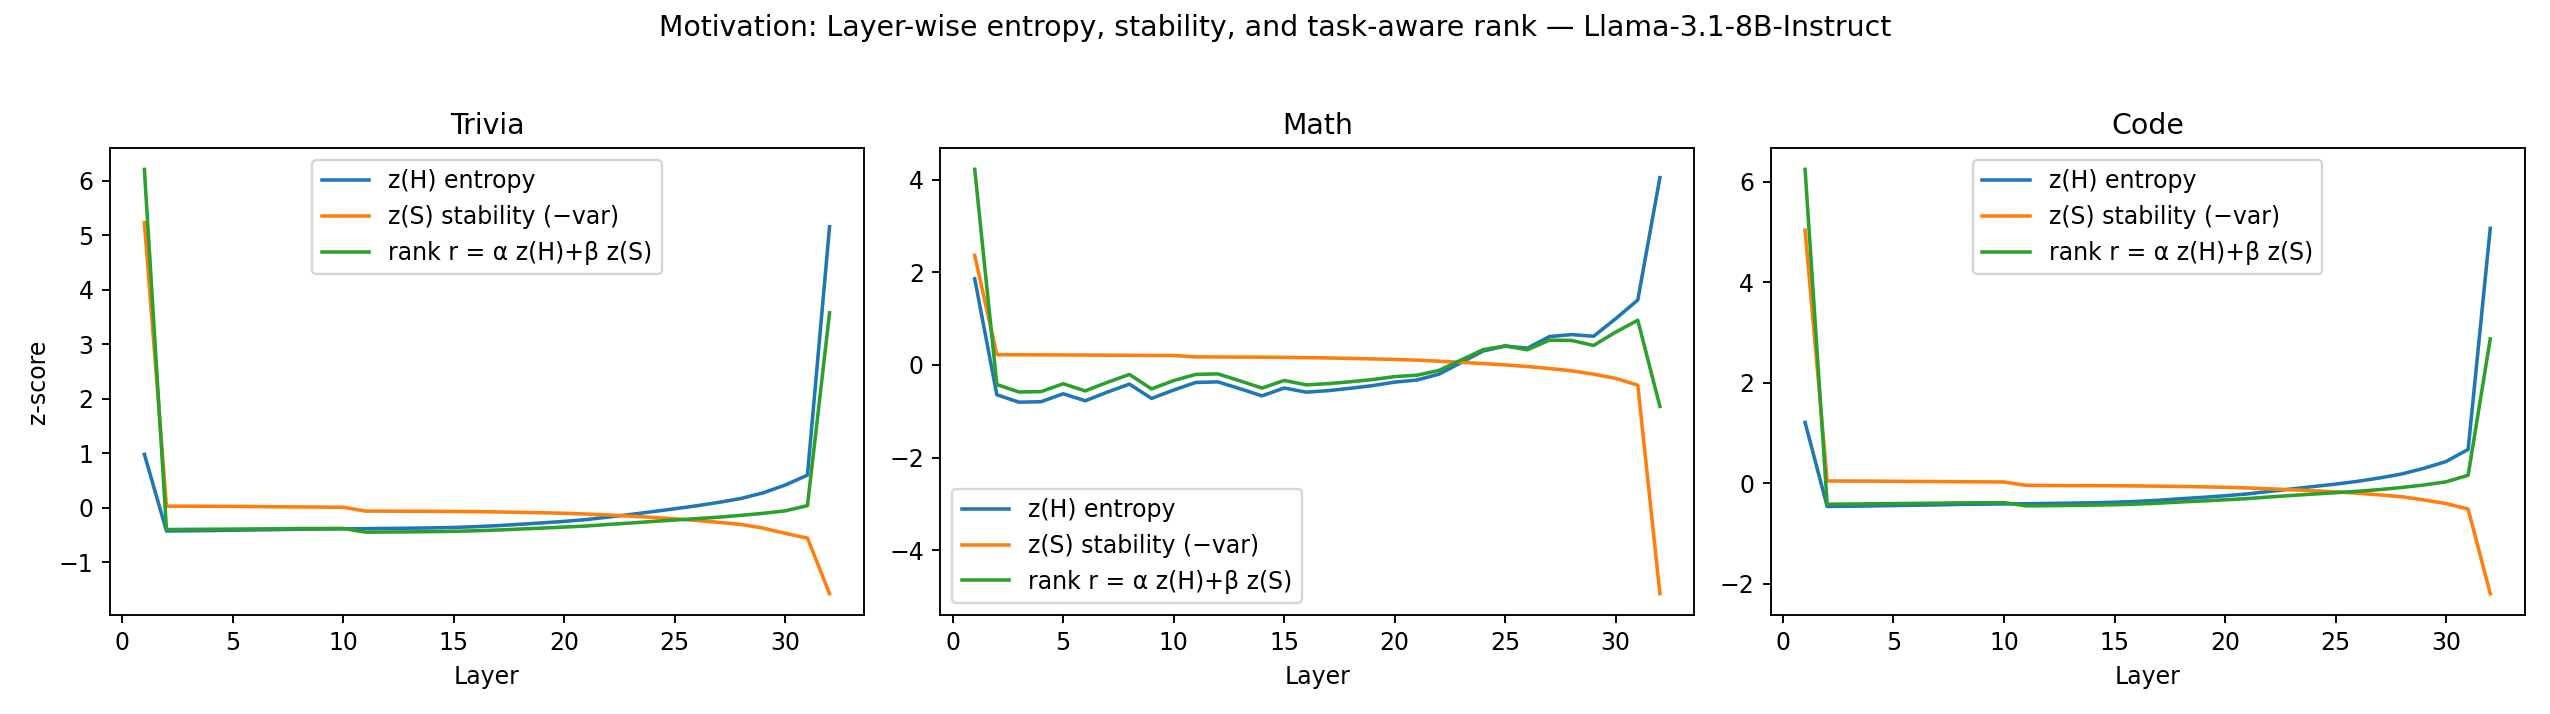
\includegraphics[width=1\linewidth]{imgs/layer_prompt_entropy.png}
  \caption{Layers relevance scores per task.}
    \label{fig:bbq_full}
\end{figure}
% \paragraph{Motivation Example, have to include empirical, interoperability, visual demonstration of the phenomena our method based on.}
% Different tasks stress different parts of a Transformer: some layers are indispensable for capturing semantic diversity, while others can be aggressively quantized with little effect. In Figure~\ref{fig:bbq_full}, we show per-layer relevance signals for Llama-3.1-8B-Instruct across TriviaQA \citep{joshi2017triviaqa} (open-domain question answering with evidence documents), GSM8K \citep{cobbe2021training} (grade-school math word problems requiring multi-step reasoning), and MBPP \citep{austin2021program} (Python code synthesis from natural-language prompts with unit tests), measured via prompt entropy $H_\ell$, stability $S_\ell=-\mathrm{Var}(X_\ell)$, and a combined rank $r_\ell=\alpha\, z(H_\ell)+\beta\, z(S_\ell)$. The resulting profiles are task-dependent: TriviaQA and MBPP concentrate importance near input/output boundaries (early lexical grounding and late semantic control), whereas GSM8K exhibits a broad mid-to-late plateau where entropy grows and stability drops, reflecting the need to preserve intermediate reasoning structure. Mid-layers in TriviaQA and MBPP are comparatively flat and redundant, tolerating more aggressive quantization. Relevance is therefore neither uniform nor universal, motivating task-aware allocation that assigns higher precision where task-specific signals concentrate.